\documentclass[8pt,xcolor=dvipsnames,compress]{beamer}
\usepackage{multimedia}
\usepackage{pcelab_theme}
\usepackage{mathtools}
\usepackage{multirow}
\usepackage{graphicx}
\usepackage{pcelab_style}
\usepackage{hyperref}
%\usepackage[algoruled,longend]{algorithm2e}
\usepackage{array}
\usepackage{graphicx}
\graphicspath{ {./images/} }
\usepackage{amsmath}
\newcolumntype{C}{>{\centering\arraybackslash} m{1000.3in} }
\newcolumntype{M}{>{\centering\arraybackslash} m{1000.in} }
\everymath{\displaystyle}
\long\def\/*#1*/{}

%\beamertemplatenavigationsymbolsempty
%\usepackage[square,numbers]{natbib}
\usepackage{tcolorbox}
\usepackage{rotating}
\usepackage{xcolor}
\usepackage[export]{adjustbox}
\usepackage{caption}
\usepackage{subcaption}
\newcommand{\bs}{\boldsymbol}
\newcommand{\thetab}{\boldsymbol\theta}

%===============================================================================
% 					 Presentation Title and Author  
%===============================================================================
\title[Fall,2019]{
TCN Implementation Example Pytorch}
\subtitle{Semester: Summer, 2024}

\author{Md Azharul Islam}

\institute[UB]{Advisor:  Dr. Danial Faghihi\\University at Buffalo\\}
    \titlegraphic{
\includegraphics[width=3cm]{PCE_logo1.png}}

\date[\today]{\today}


\begin{document}
% \titlegraphic{\hfill\includegraphics[height=1.5cm]{logo.pdf}}
\maketitle




\begin{frame}[fragile]{Bayesian TCN}
\footnotesize

\begin{figure}[htpb]
    \centering
    \begin{subfigure}[b]{0.65\textwidth}
        \centering
        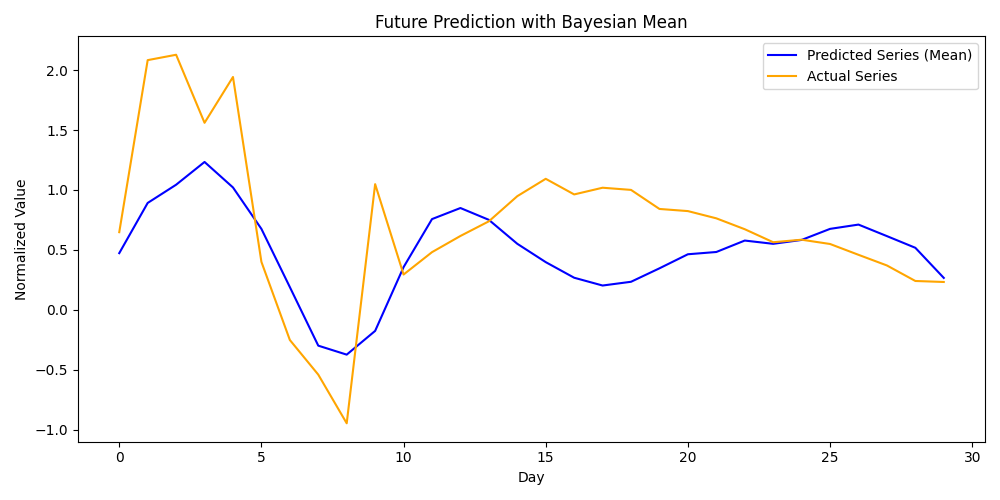
\includegraphics[scale=0.28]{figures1/predictions.png}
        \caption{30 Days prediction with variational inference}        
    \end{subfigure}
    \begin{subfigure}[b]{0.65\textwidth}
        \centering
        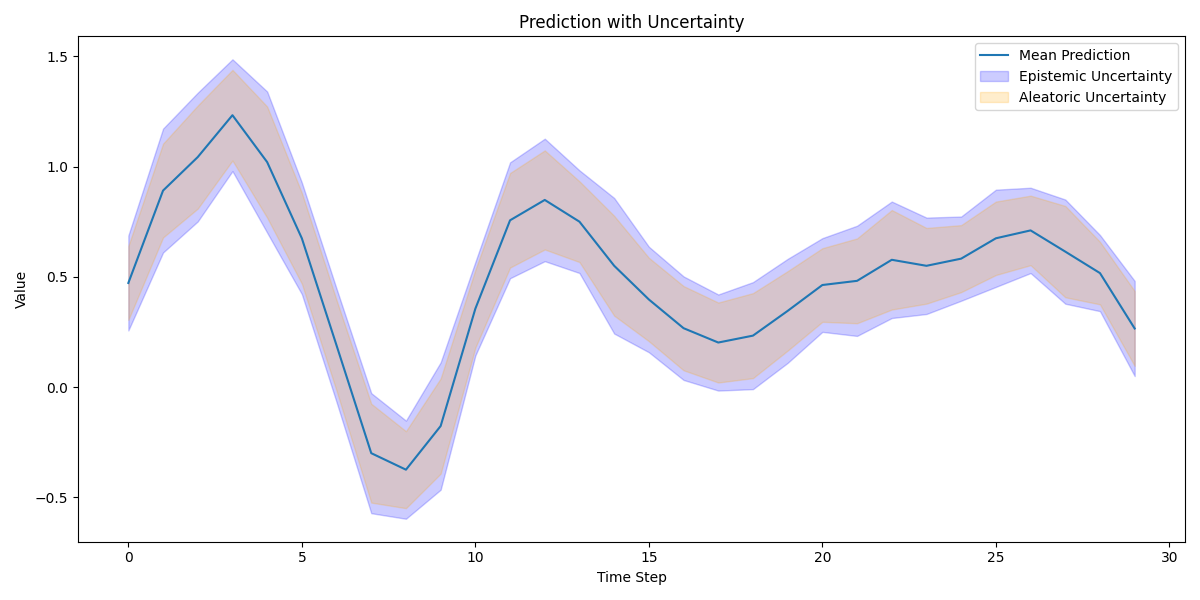
\includegraphics[scale=0.25]{figures1/uncertainty.png}
        \caption{30 days prediction with plain TCN}
    \end{subfigure}
    \label{fig:eigenvalue_decay}
\end{figure}

\end{frame}

\end{document}